\chapter{Sistemas de equações diferenciais ordinárias}
\section{Transformada de Laplace para resolver sistemas}
O método de transformada de Laplace pode ser aplicado para resolver sistemas de equações diferenciais. Para isso, aplica-se a transformada de Laplace a todas equações envolvidas, levando o sistema de equações diferenciais em um sistema de equações algébricas. Depois de resolver o sistema de equações algébricas no espaço de transformadas, calcula-se as transformadas inversas para obter a solução.
\begin{ex}Vamos resolver o seguinte problema de valor inicial:
\begin{eqnarray*}
y'&=&x\\
x'&=&y\\
x(0)&=&0\\
y(0)&=&1.
\end{eqnarray*}
Aplicamos a transformada de Laplace em cada uma das equações:
\begin{eqnarray*}
sY(s)-y(0)&=&X(s)\\
sX(s)-x(0)&=&Y(s),
\end{eqnarray*}
onde usamos a propriedade \ref{prop_der} e a notação $X(s)=\mathcal{L}\{x(t)\}$ e $Y(s)=\mathcal{L}\{y(t)\}$. Substituímos as condições iniciais para obter o seguinte sistema de equações algébricas
\begin{eqnarray}
\label{sis_eq_1}-X(s)+sY(s)&=&1\\
\label{sis_eq_2} sX(s)-Y(s)&=&0.
\end{eqnarray}
Multiplicamos a equação (\ref{sis_eq_1}) por $s$, $-sX(s)+s^2Y(s)=s$, e somamos com a equação (\ref{sis_eq_2}) para obter
\begin{equation}
(s^2-1)Y(s)=s.
\end{equation}
Logo
\begin{equation}
Y(s)=\frac{s}{s^2-1}.
\end{equation}
Resolvemos $X(s)$ usando a equação (\ref{sis_eq_2}):
\begin{equation}
X(s)=\frac{Y(s)}{s}=\frac{1}{s^2-1}.
\end{equation}
As transformadas inversas de $X(s)$ e $Y(s)$ estão tabeladas:
\begin{eqnarray*}
x(t)&=&\senh(t)\\
y(t)&=&\cosh(t).
\end{eqnarray*}
\end{ex}
\begin{ex}Considere o seguinte problema de valor inicial:
\begin{eqnarray*}
2\frac{d^2x}{dt^2}+\frac{d^2y}{dt^2}&=&t^2\\
\frac{d^2x}{dt^2}-\frac{d^2y}{dt^2}&=&4t\\
x(0)&=&2\\
x'(0)&=&0\\
y(0)&=&-1\\
y'(0)&=&10.
\end{eqnarray*}
Aplicamos a transformada de Laplace em cada uma das equações:
\begin{eqnarray*}
2s^2X(s)-2sx(0)-2x'(0)+s^2Y(s)-sy(0)-y'(0)&=&\frac{2}{s^3}\\
s^2X(s)-sx(0)-x'(0)-s^2Y(s)+sy(0)+y'(0)&=&\frac{4}{s^2},
\end{eqnarray*}
onde usamos a propriedade \ref{prop_der} e a notação $X(s)=\mathcal{L}\{x(t)\}$ e $Y(s)=\mathcal{L}\{y(t)\}$. Substituímos as condições iniciais para obter o seguinte sistema de equações algébricas
\begin{eqnarray*}
2s^2X(s)-4s+0+s^2Y(s)+s-10&=&\frac{2}{s^3}\\
s^2X(s)-2s+0-s^2Y(s)-s+10&=&\frac{4}{s^2}.
\end{eqnarray*}
ou seja,
\begin{eqnarray}
\label{sis_eq_3}2s^2X(s)+s^2Y(s)&=&\frac{2}{s^3}+10+3s\\
\label{sis_eq_4} s^2X(s)-s^2Y(s)&=&\frac{4}{s^2}-10+3s.
\end{eqnarray}
A soma das equações (\ref{sis_eq_3}) e (\ref{sis_eq_4}) resulta em
\begin{equation}
3s^2X(s)=\frac{2}{s^3}+\frac{4}{s^2}+6s.
\end{equation}
Logo,
\begin{equation}
X(s)=\frac{2}{3s^5}+\frac{4}{3s^4}+\frac{2}{s}.
\end{equation}
Agora, usamos (\ref{sis_eq_4}) para resolver $Y(s)$:
\begin{equation}
s^2\left(\frac{2}{3s^5}+\frac{4}{3s^4}+\frac{2}{s}\right)-s^2Y(s)=\frac{4}{s^2}-10+3s.
\end{equation}
Assim,
\begin{equation}
Y(s)=\frac{2}{3s^5}-\frac{8}{3s^4}+\frac{10}{s^2}-\frac{1}{s}.
\end{equation}
As transformadas inversas estão tabeladas:
\begin{eqnarray*}
x(t)&=&\frac{t^4}{36}+\frac{2t^3}{9}+2\\
y(t)&=&\frac{t^4}{36}-\frac{4t^3}{9}+10t-1.
\end{eqnarray*}
\end{ex}


\section{Aplicação: circuito de duas malhas}
Considere o circuito da figura \ref{fig_circ_2_malha}, constituído de duas malhas com correntes $i_1$ e $i_2$, respectivamente. Vamos modelar $i_1$ e $i_2$ considerando $i_1(0)=i_2(0)=0$. 
\begin{figure}[!ht]
\begin{center}

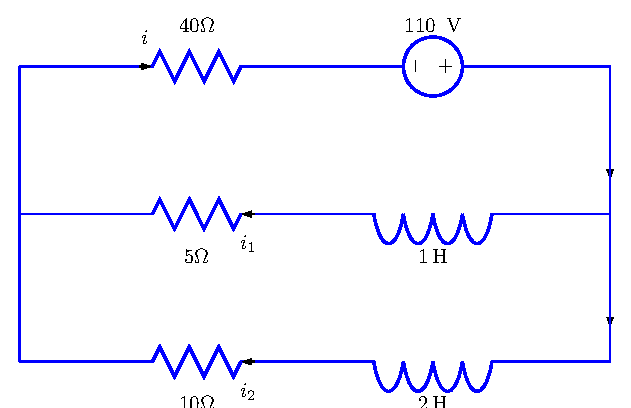
\includegraphics{cap_sistemas/pics/figura_1}\end{center}
\caption{\label{fig_circ_2_malha}}
\end{figure}
Usamos a lei de Kirchoff para obter
\begin{eqnarray*}
\frac{di_1(t)}{dt}+5i_1(t)+40i(t)&=&110\\
2\frac{di_2(t)}{dt}+10i_2(t)+40i(t)&=&110 .
\end{eqnarray*}
Usando $i(t)=i_1(t)+i_2(t)$, temos
\begin{eqnarray*}
\frac{di_1(t)}{dt}+45i_1(t)+40i_2(t)&=&110\\
2\frac{di_2(t)}{dt}+40i_1(t)+50i_2(t)&=&110 ,
\end{eqnarray*}
ou simplesmente
\begin{eqnarray*}
\frac{di_1(t)}{dt}+45i_1(t)+40i_2(t)&=&110\\
\frac{di_2(t)}{dt}+20i_1(t)+25i_2(t)&=&55 .
\end{eqnarray*}
Aplicamos a transformada de Laplace e obtemos:
\begin{eqnarray*}
sI_1(s)-i_1(0)+45I_1(s)+40I_2(s)&=&\frac{110}{s}\\
sI_2(s)-i_2(0)+20I_1(s)+25I_2(s)&=&\frac{55}{s} .
\end{eqnarray*}
ou seja,
\begin{eqnarray*}
\left(s+45\right) I_1(s)+40I_2(s)&=&\frac{110}{s}\\
20I_1(s)+\left(s+25\right)I_2(s)&=&\frac{55}{s} .
\end{eqnarray*}
ou, ainda,
\begin{equation*}
\left[\begin{array}{cc}  \left(s+45\right) &40\\20& \left(s+25\right) \end{array}\right]\left[\begin{array}{c}I_1(s)\\I_2(s)\end{array}\right]=\left[\begin{array}{c}\frac{110}{s}\\ \\
\frac{55}{s}\end{array}\right]
\end{equation*}
A solução desse sistema é dada por
\begin{equation*}
\left[\begin{array}{c}I_1(s)\\I_2(s)\end{array}\right]=\frac{1}{(s+25)(s+45)-800}\left[\begin{array}{cc}  \left(s+25\right) &-40\\-20& \left(s+45\right) \end{array}\right]\left[\begin{array}{c}\frac{110}{s}\\ \\
\frac{55}{s}\end{array}\right]
\end{equation*}
Portanto,
\begin{equation}
I_1(s)=\frac{1}{s^2+70s+325}\left(\frac{110}{s}(s+25)-\frac{2200}{s}\right)=\frac{1}{(s+5)(s+65)}\left(110+\frac{550}{s}\right)
\end{equation}
e
\begin{equation}
I_2(s)=\frac{1}{s^2+70s+325}\left(-\frac{2200}{s}+\frac{55}{s}(s+45)\right)=\frac{1}{(s+5)(s+65)}\left(55+\frac{275}{s}\right).
\end{equation}
Aqui percebemos que $I_1(s)=2I_2(s)$ e, assim, vamos calcular apenas $I_2(s)$: 
\begin{equation}
I_2=\frac{1}{(s+5)(s+65)}\left(\frac{55s+275}{s}\right)=\frac{55}{(s+5)(s+65)}\left(\frac{s+5}{s}\right)=\frac{55}{s(s+65)}.
\end{equation}
Logo,
\begin{equation}
i_2(t)=\frac{55}{65}\left(1-e^{-65t}\right)=\frac{11}{13}\left(1-e^{-65t}\right).
\end{equation}
Como $i_1(t)=2i_2(t)$, temos:
\begin{equation}
i_1(t)=\frac{22}{13}\left(1-e^{-65t}\right).
\end{equation}



\section{Aplicação: duplo massa mola}
Considere o duplo sistema massa-mola, onde as molas possuem constantes $k_1$ e $k_2$ e as massas envolvidas são $m_1$ e $m_2$. Desconsiderando o amortecimento, temos o seguinte sistema:
\begin{eqnarray*}
 m_1 \ddot{x}_1(t) &=&  - k_1 x_1(t) + k_2\left[x_2(t)-x_1(t)\right]+f_1(t)\\
 m_2 \ddot{x}_2(t) &=&  - k_2\left[x_2(t)-x_1(t)\right]+f_2(t),
\end{eqnarray*}
onde $x_1$ e $x_2$ representam o deslocamento de cada uma das massas e $f_1$ e $f_2$ são as forças externas aplicadas. Tomando transformada de Laplace, obtemos:
\begin{eqnarray*}
 m_1 (s^2X_1(s)-\dot{x}_1(0)-sx_1(0)) &=&  - (k_1+k_2) X_1(s) + k_2X_2(s)+F_1(s)\\
 m_2 (s^2X_2(s)-\dot{x}_2(0)-sx_2(0)) &=&  - k_2X_2(s)+k_2X_1(s)+F_2(s)
\end{eqnarray*}
isto é:
\begin{eqnarray*}
 \left(m_1 s^2+k_1+k_2\right)X_1(s)- k_2X_2(s) &=&   F_1(s)+m_1\dot{x}_1(0)+sm_1x_1(0)\\
 -k_2X_1(s)+\left(m_2 s^2+k_2\right)X_2(s) &=&  F_2(s)+m_2\dot{x}_2(0)+sm_2x_2(0)
\end{eqnarray*}
A representação matricial do sistema é:
\begin{eqnarray*}
\left[\begin{array}{cc}
       m_1 s^2+k_1+k_2 &- k_2\\
 -k_2&      m_2 s^2+k_2
      \end{array}
\right]
\left[\begin{array}{c}
       X_1(s)\\
       X_2(s)
      \end{array}
\right]=\left[\begin{array}{c}
F_1(s)+m_1\dot{x}_1(0)+sm_1x_1(0)\\  
F_2(s)+m_2\dot{x}_2(0)+sm_2x_2(0)
       \end{array}
\right]
\end{eqnarray*}
e sua solução pode ser escrita como:
\begin{eqnarray}{\label{eq_transf_2_massa_mola}}
\left[\begin{array}{c}
       X_1(s)\\
       X_2(s)
      \end{array}
\right]
&=&\frac{1}{P(s)}
\left[\begin{array}{cc}
       m_2s^2+k_2 & k_2\\
 k_2&      m_1 s^2+k_1+k_2
      \end{array}
\right]
\left[\begin{array}{c}
F_1(s)+m_1\dot{x}_1(0)+sm_1x_1(0)\\  
F_2(s)+m_2\dot{x}_2(0)+sm_2x_2(0)
       \end{array}
\right],
\end{eqnarray}
onde $P(s)=m_1m_2s^4+(m_1k_2+m_2k_1+m_2k_2)s^2+k_1k_2$. Vamos resolver um caso particular onde $m_1=m_2=1$, $f_1=f_2=0$, $k_1=6$ e $k_2=4$, temos o seguinte sistema massa-mola:
\begin{eqnarray*}
  \ddot{x}_1(t) &=&  - 6 x_1(t) + 4\left[x_2(t)-x_1(t)\right]\\
 \ddot{x}_2(t) &=&  - 4\left[x_2(t)-x_1(t)\right],
\end{eqnarray*}
Usando (\ref{eq_transf_2_massa_mola}), temos:
\begin{eqnarray*}
\left[\begin{array}{c}
       X_1(s)\\
       X_2(s)
      \end{array}
\right]
&=&\frac{1}{s^4+14s^2+24}
\left[\begin{array}{cc}
       s^2+4 & 4\\
 4&       s^2+10
      \end{array}
\right]
\left[\begin{array}{c}
\dot{x}_1(0)+sx_1(0)\\  
\dot{x}_2(0)+sx_2(0)
       \end{array}
\right].
\end{eqnarray*}
Para completar o sistema, impondo as seguintes condições iniciais: $x_1(0)=x_2(0)=0$, $\dot{x}_1(0)=1$ e $\dot{x}_2(0)=-1$:
\begin{eqnarray*}
\left[\begin{array}{c}
       X_1(s)\\
       X_2(s)
      \end{array}
\right]
&=&\frac{1}{s^4+14s^2+24}
\left[\begin{array}{cc}
       s^2+4 & 4\\
 4&       s^2+10
      \end{array}
\right]
\left[\begin{array}{c}
1\\  
-1
       \end{array}
\right].
\end{eqnarray*}
Logo,
\begin{equation}
X(s)=\frac{1}{s^4+14s^2+24}\left(s^2+4-4\right)=\frac{s^2}{s^4+14s^2+24}
\end{equation}
e
\begin{equation}
X(s)=\frac{1}{s^4+14s^2+24}\left(4-s^2-10\right)=\frac{-s^2-6}{s^4+14s^2+24}.
\end{equation}
Usamos frações parciais para escrever
\begin{eqnarray*}
\frac{s^2}{s^4+14s^2+24}=\frac{s^2}{(s^2+2)(s^2+12)}&=&\frac{A}{s^2+2}+\frac{B}{s^2+12}\\&=&\frac{A(s^2+12)+B(s^2+2)}{(s^2+2)(s^2+12)}\\
&=&\frac{(A+B)s^2+12A+2B}{(s^2+2)(s^2+12)},
\end{eqnarray*}
ou seja, $A+B=1$ e $12A+2B=0$. Logo, $B=-6A$ e $A-6A=1$, ou seja, $A=-\frac{1}{5}$ e $B=\frac{6}{5}$. Portanto,
\begin{equation}
X(s)=\frac{1}{5}\left(\frac{6}{s^2+12}-\frac{1}{s^2+2}\right)=\frac{6}{5\sqrt{12}}\frac{\sqrt{12}}{s^2+\sqrt{12}^2}-\frac{1}{5\sqrt{2}}\frac{\sqrt{2}}{s^2+\sqrt{2}^2},
\end{equation}
e, calculando a transformada inversa, temos:
\begin{eqnarray*}
x(t)&=&\frac{6}{5\sqrt{12}}\sen(\sqrt{12}t)-\frac{1}{5\sqrt{2}}\sen(\sqrt{2}t)\\
&=&\frac{\sqrt{3}}{5}\sen(2\sqrt{3}t)-\frac{\sqrt{2}}{10}\sen(\sqrt{2}t).
\end{eqnarray*}
Da mesma forma,
\begin{equation}
Y(s)=-\frac{3}{5}\left(\frac{1}{s^2+12}-\frac{2}{5}\frac{1}{s^2+2}\right)=-\frac{3}{5\sqrt{12}}\frac{\sqrt{12}}{s^2+\sqrt{12}^2}-\frac{2}{5\sqrt{2}}\frac{\sqrt{2}}{s^2+\sqrt{2}^2},
\end{equation}
e
\begin{eqnarray*}
y(t)&=&-\frac{3}{5\sqrt{12}}\sen(\sqrt{12}t)-\frac{2}{5\sqrt{2}}\sen(\sqrt{2}t)\\
&=&-\frac{\sqrt{3}}{10}\sen(2\sqrt{3}t)-\frac{\sqrt{2}}{5}\sen(\sqrt{2}t).
\end{eqnarray*}
A figura \ref{fig_massa_mola_2_malha} apresenta os gráficos de $x(t)$ e $y(t)$:
 \begin{figure}[!ht]
\begin{center}

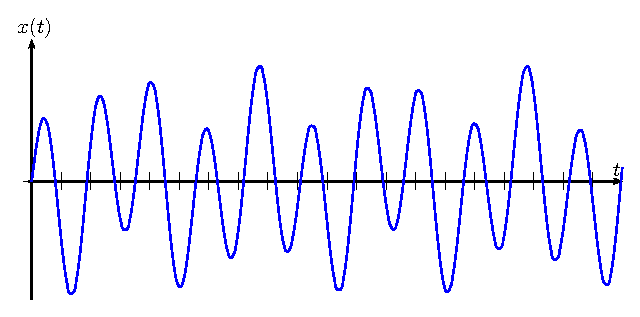
\includegraphics{cap_sistemas/pics/figura_2}
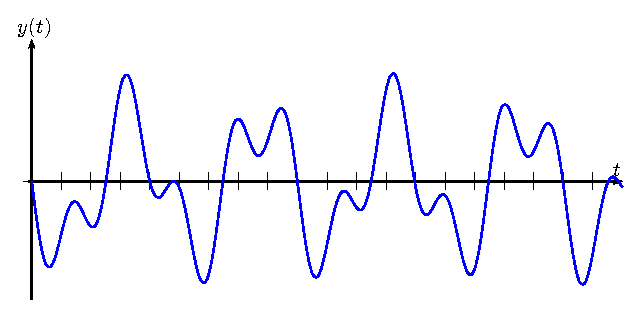
\includegraphics{cap_sistemas/pics/figura_3}\end{center}
\caption{\label{fig_massa_mola_2_malha}}
\end{figure}


\section{Aplicação: reação química}
Considere o mecanismo simplificado de reação química apresentado a seguir:
\begin{equation}R\longrightarrow S \longrightarrow T\end{equation}
onde a concentração de $R$, $S$ e $T$ são dadas em $\hbox{mol}/l$ por $x(t)$, $y(t)$ e $z(t)$, respectivamente e são regidas pelo seguinte sistema de equações diferenciais ordinárias:
\begin{eqnarray*}
x'(t)&=&-\alpha x(t) \\
y'(t)&=&\alpha x(t)-\gamma y(t)\\
z'(t)&=&\gamma y(t),
\end{eqnarray*} 
onde $\alpha$ e $\gamma$ são constantes positivas. Sabendo que as concentrações iniciais são dadas por:
\begin{equation}x(0)=1,~~~~ y(0)=z(0)=0.\end{equation}
Usando a teoria das Transformadas de Laplace, vamos obter a solução dada pelas funções $x(t)$, $y(t)$ e $z(t)$ quando $\alpha=1$, e $\gamma=2$. Calculamos a Transformada de Laplace do sistema usando a propriedade da linearidade \ref{prop_lin} e da derivada \ref{prop_der}:
\begin{eqnarray*}
sX(s)-x(0)&=&-\alpha X(s) \\
sY(s)-y(0)&=&\alpha X(s)-\gamma Y(s)\\
sZ(s)-z(0)&=&\gamma Y(s).
\end{eqnarray*} 
Da primeira equação, temos:
\begin{equation}
\label{eqX}X(s)=\frac{x(0)}{s+\alpha}=\frac{1}{s+1}.
\end{equation}
Da segunda equação, temos:
\begin{equation}
Y(s)=\frac{\alpha X(s)}{s+\gamma}=\frac{\alpha x(0) }{(s+\gamma)(s+\alpha)}=\frac{1}{(s+1)(s+2)}.
\end{equation}
Da terceira equação temos:
\begin{equation}
Z(s)=\frac{\gamma Y(s)}{s}=\frac{2}{s(s+1)(s+2)}.
\end{equation}
Agora, podemos obter as funções $x(t)$, $y(t)$ e $z(t)$ através da Transformada Inversa de Laplace:
\begin{equation}
x(t)=\mathcal{L}^{-1}\left\{X(s)\right\}=e^{-t}
\end{equation}
onde usamos item 7 da tabela \ref{tab_trans_Lap_1};
\begin{equation}
y(t)=\mathcal{L}^{-1}\left\{Y(s)\right\}=-e^{-2t}+e^{-t},
\end{equation}
onde usamos item 11 da tabela \ref{tab_trans_Lap_1} com $a=2$ e $b=-1$;
\begin{eqnarray*}
z(t)=\mathcal{L}^{-1}\left\{Z(s)\right\}&=&2\mathcal{L}^{-1}\left\{\frac{Y(s)}{s}\right\}\\&=&2\int_0^ty(\tau)d\tau\\
&=&2\int_0^t\left(-e^{-2\tau}+e^{-\tau}\right)d\tau\\&=&2\left(\frac{e^{-2t}-1}{2}-\left(e^{-t}-1\right)\right)\\&=&e^{-2t}-2e^{-t}+1,
\end{eqnarray*}
 onde usamos a propriedade da convolução \ref{prop_conv} na passagem da primeira para a segunda linha. A figura \ref{reacao} apresenta o gráfico de das funções $x(t)$, $y(t)$ e $z(t)$.
 \begin{figure}[!ht]
\begin{center}

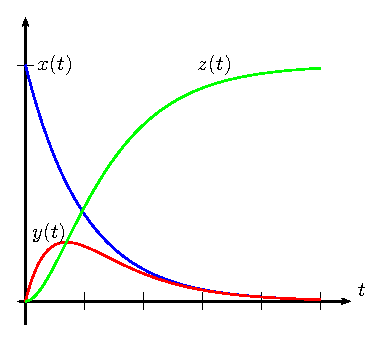
\includegraphics{cap_sistemas/pics/figura_4}\end{center}
\caption{\label{reacao}}
\end{figure}



\subsection*{Exercícios}
\begin{exer}
Considere o seguinte problema de valor inicial:
\begin{eqnarray*}
x'(t)&=&-2x(t) +  y(t)\\
y'(t)&=&\alpha x(t) - 2y(t)\\
\end{eqnarray*}
Com $x(0)=0$ e $y(0)=3$, onde $\alpha$ é uma constante real.
\begin{itemize}
 \item[a)] Assinale a alternativa que indica o tipo de amortecimento do sistema dado para os valores de $\alpha$ dados respectivamente por $-1$, $0$, $1$ e $2$:
 \subitem(~~) Sem amortecimento, subamortecido, criticamente amortecido e superamortecido.
 \subitem(~~) Subamortecido, subamortecido, criticamente amortecido e superamortecido.
 \subitem(~~) Subamortecido, criticamente amortecido, superamortecido e superamortecido.
 \subitem(~~) Superamortecido, superamortecido, criticamente amortecido e subamortecido.
 \subitem(~~) Superamortecido, criticamente amortecido, subamortecido e subamortecido.
 \subitem(~~) Superamortecido, criticamente amortecido, subamortecido e sem amortecimento.
\item [b)] Use a técnica da Transformada de Laplace para encontrar uma expressão para $x(t)$ e $y(t)$ quando $\alpha=1$. 
\end{itemize}
\end{exer}
\begin{exer}A temperatura em um forno industrial evolui no tempo conforme o seguinte modelo simplificado:
\begin{equation}\frac{d u(t)}{dt}=-\lambda (u(t)-u_{amb}) + q(t)\end{equation}
onde $u(t)$ representa a temperatura medida no forno, $u_{amb}$ é temperatura ambiente, considerada constante, $q(t)$ é a potência de aquecimento e $\lambda$ é uma constante relacionada às trocas de calor. Considere $u(0)=50$, $u_{amb}=50$ e $\lambda=4$. Usando a técnicas das transformadas de Laplace, faça o que se pede:
\begin{itemize}
 \item [a)] Mostre que $U(s)=\frac{50}{s}+\frac{Q(s)}{s+4}$.
 \item [b)] Calcule a temperatura $u(t)$ quando  $q(t)=100 \delta(t-1)$. Esboce o gráfico de $u(t)$.
 \item [c)] Suponha, agora, que a temperatura é regulada por um sistema de controle automático que aumenta a potência $q(t)$ sempre que a temperatura está abaixo da temperatura de ajuste e reduz a potência sempre que a temperatura se encontra acima da temperatura de ajuste. O sistema de controle automático reage conforme a seguinte equação:
 \begin{equation}\frac{dq(t)}{dt} = \eta (u_a-u(t)).\end{equation}
 onde $u_a$ é a temperatura de ajuste e $\eta$ é uma constante positiva. Calcule o valor de $\eta$ para que o sistema resultante do acoplamente entre o modelo do forno e o sistema de controle automático seja criticamente amortecido. Mostre que $U(s)=\frac{200}{s}-\frac{150}{s+2}-\frac{300}{(s+2)^2}+\frac{q(0)}{(s+2)^2}$.
 \item[d)] Use a propriedade do valor final para obter $\displaystyle\lim_{t\to+\infty} u(t)$ no item c).
 \item[e)] Resolva o problema acoplado usando a constante $\eta$ calculada no item c, considerando $u_a=200$ e $q(0)=600$.
  \item[f)] Observe que a solução obtida no item e) satisfaz a condição inicial e tem a propriedade $\displaystyle\lim_{t\to \infty}u(t)=u_a$. Verifique também que $q(0)=\lim_{t\to+\infty} q(t)$.
 \item [g)] Esboce o gráfico da $u(t)$ obtida no item d).
 \end{itemize}
\end{exer}
\begin{resp}
\begin{itemize}
 \item [a)] Observe que $U(s)=\frac{50}{s+4}+\frac{200}{s(s+4)}+\frac{100}{s+4}e^{-s}$ pode ser escrito como $U(s)=\frac{50}{s}+\frac{100}{s+4}e^{-s}$ 
  \item [b)] $u(t)=50+100u(t-1)e^{-4(t-1)}$.
  \begin{center}

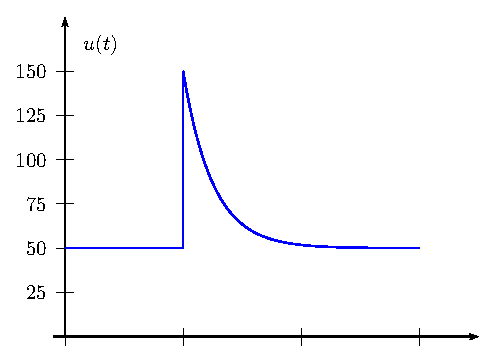
\includegraphics{cap_sistemas/pics/figura_5}\end{center}
  \item [c)] $\eta=4$
 \item [d)] 200
 \item[e)] $u(t)=200-150e^{-2t}\left(1+2t\right)$
 \item [g)] 
\end{itemize}
\begin{center}

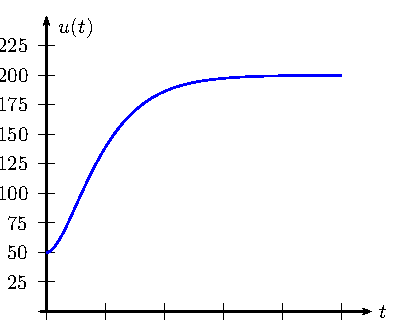
\includegraphics{cap_sistemas/pics/figura_6}\end{center}
\end{resp}
\begin{exer} Considere o seguinte problema de valor inicial para um sistema de equações integro-diferenciais:
\begin{eqnarray*}
 x'(t) +x(t) = 2 y(t)\\
 x(t) = \int_0^t y(\tau) d\tau + 1
\end{eqnarray*}
com $x(0)=0$. Usando a teoria das Transformadas de Laplace, resolve o sistema, obtendo $x(t)$ e $y(t)$.
{\bf Obs:}  Este sistema apresenta ``problemas na origem''. 
\end{exer}
\begin{resp}
 \begin{eqnarray}
  x(t)&=&2e^t  \\
  y(t)&=&\delta(t)+e^t
 \end{eqnarray}
\end{resp}


\begin{exer}
Considere o seguinte problema de valor inicial:
 \begin{eqnarray*}
x'(t)&=&- x(t) -2 y(t)+\delta(t)\\
y'(t)&=& x(t) - y(t)+\delta(t),
\end{eqnarray*}
com $x(0)=0$ e $y(0)=0$.\\
 \indent  {a)}  Calcule as transformadas de Laplace $X(s)=\mathcal{L}\{x(t)\}$ e $Y(s)=\mathcal{L}\{y(t)\}$.
 \indent  {b)}  Calcule as transformadas inversas de Laplace $x(t)$ e $y(t)$.
\indent  {c)} Aplique sua solução do item b) nas condições inciais e justifique o resultado encontrado.\\

\end{exer}